
% This LaTeX was auto-generated from MATLAB code.
% To make changes, update the MATLAB code and republish this document.

\documentclass{article}
\usepackage{graphicx}
\usepackage{color}

\sloppy
\definecolor{lightgray}{gray}{0.5}
\setlength{\parindent}{0pt}

\begin{document}

    
    
\subsection*{Contents}

\begin{itemize}
\setlength{\itemsep}{-1ex}
   \item Task 1
   \item Task 2
   \item Task 3
\end{itemize}


\subsection*{Task 1}


        \color{lightgray} \begin{verbatim}
h = 

  HeatmapChart with properties:

        XData: {5�1 cell}
        YData: {5�1 cell}
    ColorData: [5�5 double]

  Use GET to show all properties

\end{verbatim} \color{black}
    
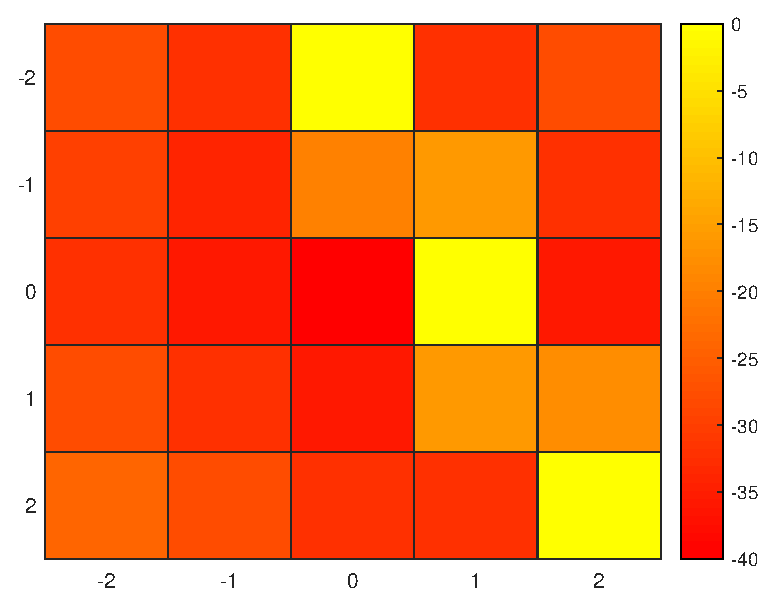
\includegraphics [width=4in]{assign3_part2_01.eps}

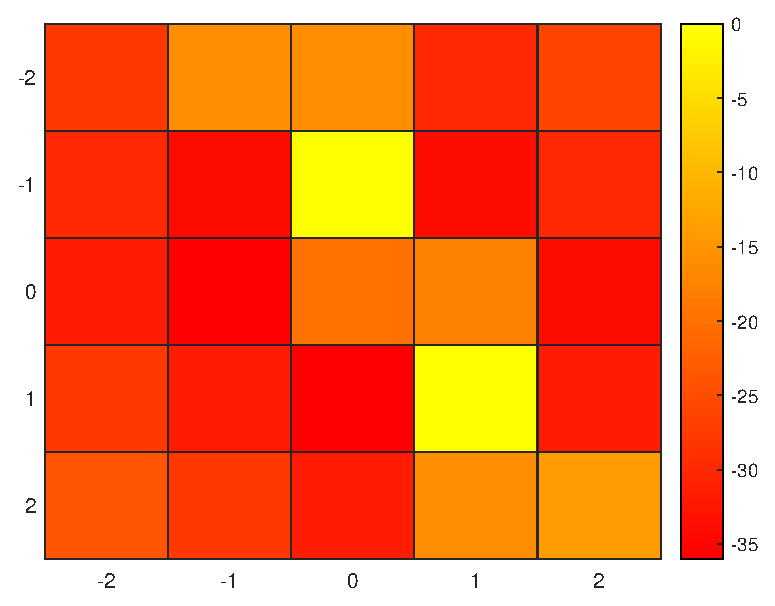
\includegraphics [width=4in]{assign3_part2_02.eps}

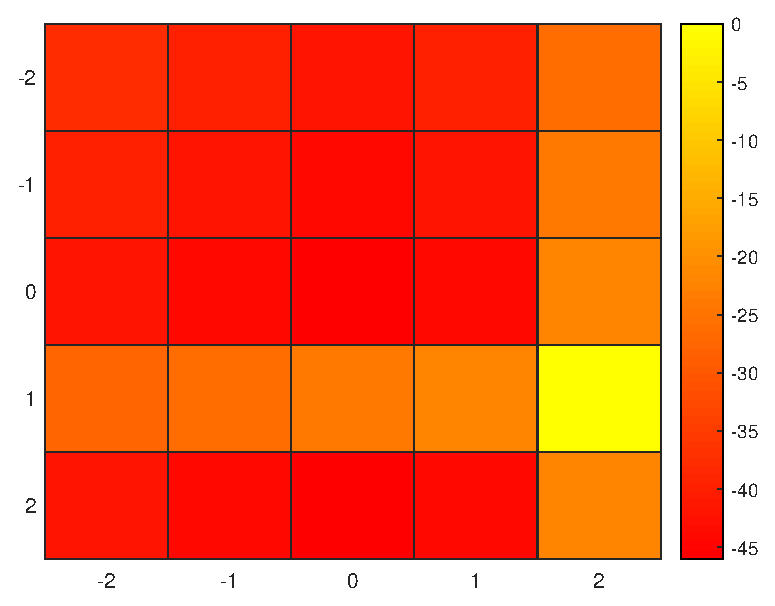
\includegraphics [width=4in]{assign3_part2_03.eps}


\subsection*{Task 2}


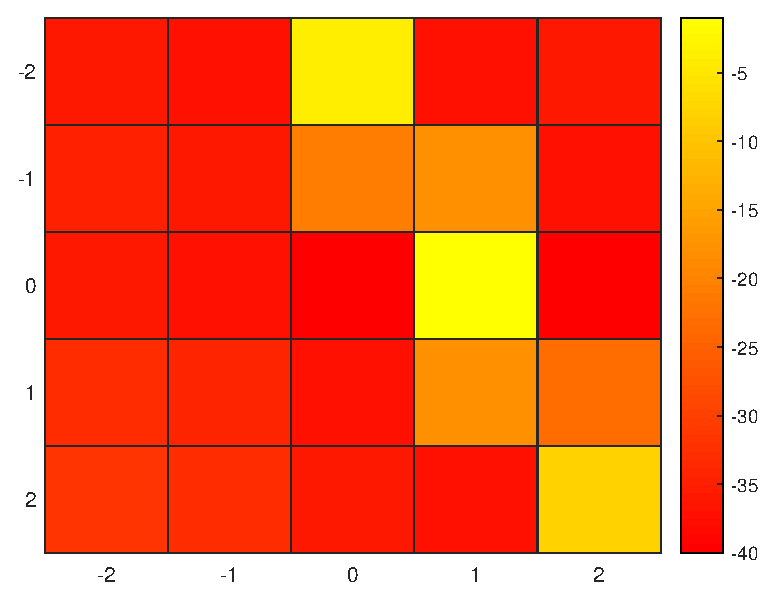
\includegraphics [width=4in]{assign3_part2_04.eps}

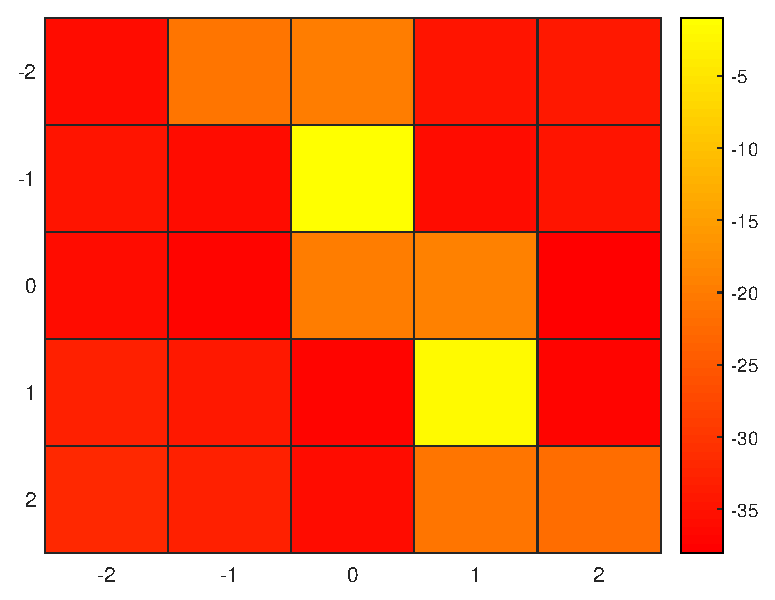
\includegraphics [width=4in]{assign3_part2_05.eps}

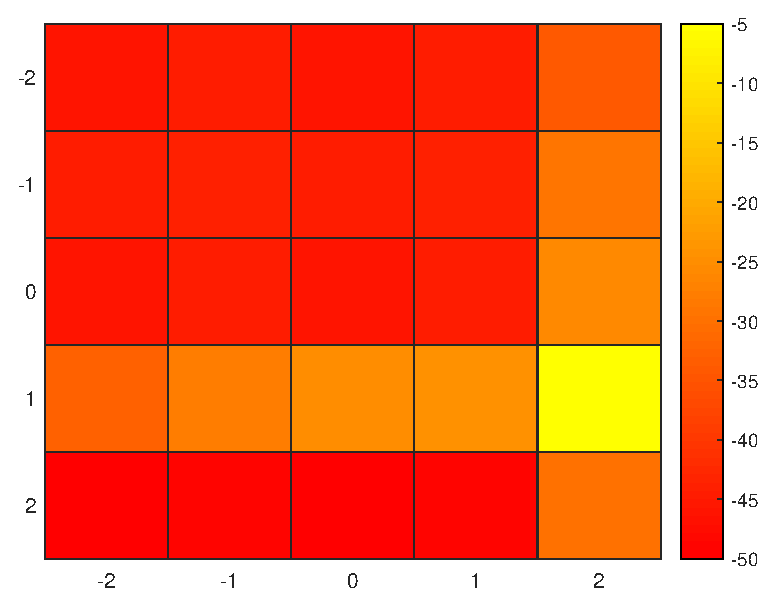
\includegraphics [width=4in]{assign3_part2_06.eps}


\subsection*{Task 3}


        \color{lightgray} \begin{verbatim}
h = 

  HeatmapChart with properties:

        XData: {5�1 cell}
        YData: {5�1 cell}
    ColorData: [5�5 double]

  Use GET to show all properties

\end{verbatim} \color{black}
    
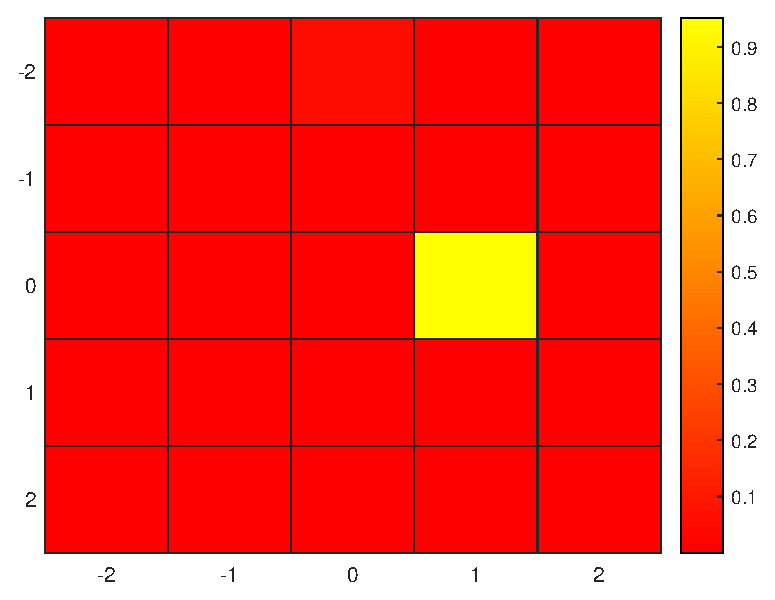
\includegraphics [width=4in]{assign3_part2_07.eps}

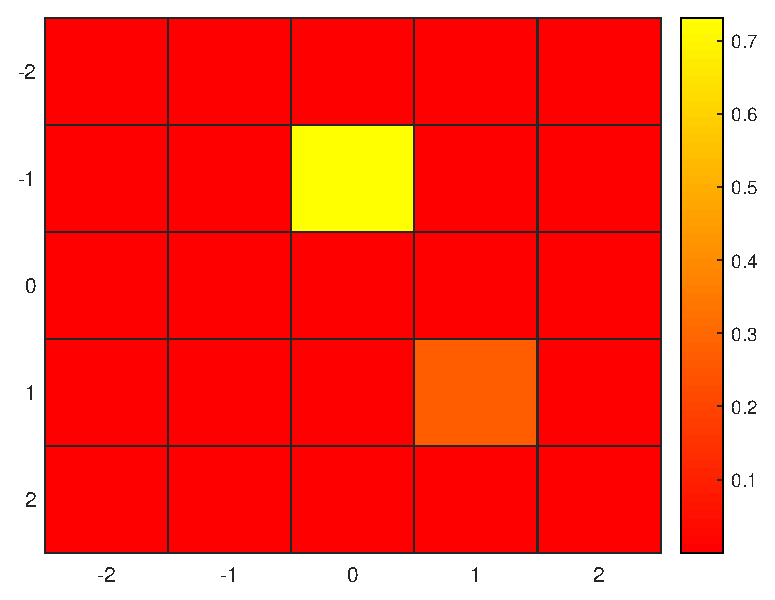
\includegraphics [width=4in]{assign3_part2_08.eps}

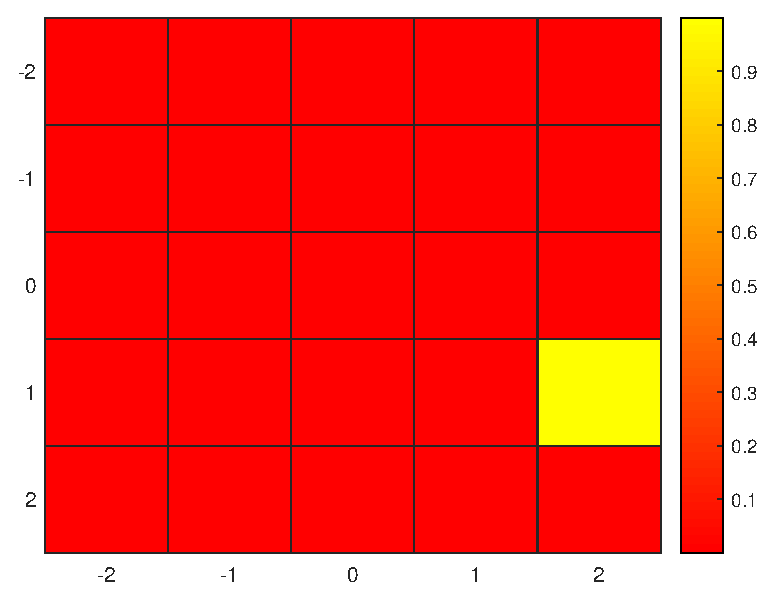
\includegraphics [width=4in]{assign3_part2_09.eps}



\end{document}
    
